%% iccp20_template.tex
%% Created by Ayan Chakrabarti from the IEEE bare_jrnl_compsoc.tex file.
%%
%% bare_jrnl_compsoc.tex
%% V1.4b
%% 2015/08/26
%% by Michael Shell
%% See:
%% http://www.michaelshell.org/
%% for current contact information.
%%
%% This is a skeleton file demonstrating the use of IEEEtran.cls
%% (requires IEEEtran.cls version 1.8b or later) with an IEEE
%% Computer Society journal paper.
%%
%% Support sites:
%% http://www.michaelshell.org/tex/ieeetran/
%% http://www.ctan.org/pkg/ieeetran
%% and
%% http://www.ieee.org/

%%*************************************************************************
%% Legal Notice:
%% This code is offered as-is without any warranty either expressed or
%% implied; without even the implied warranty of MERCHANTABILITY or
%% FITNESS FOR A PARTICULAR PURPOSE! 
%% User assumes all risk.
%% In no event shall the IEEE or any contributor to this code be liable for
%% any damages or losses, including, but not limited to, incidental,
%% consequential, or any other damages, resulting from the use or misuse
%% of any information contained here.
%%
%% All comments are the opinions of their respective authors and are not
%% necessarily endorsed by the IEEE.
%%
%% This work is distributed under the LaTeX Project Public License (LPPL)
%% ( http://www.latex-project.org/ ) version 1.3, and may be freely used,
%% distributed and modified. A copy of the LPPL, version 1.3, is included
%% in the base LaTeX documentation of all distributions of LaTeX released
%% 2003/12/01 or later.
%% Retain all contribution notices and credits.
%% ** Modified files should be clearly indicated as such, including  **
%% ** renaming them and changing author support contact information. **
%%*************************************************************************


\documentclass[10pt,journal,compsoc]{IEEEtran}
\newif\ifpeerreview

%%% Important: for camera ready submissions, replace the following line
%%% with \peerreviewfalse
\peerreviewfalse


\usepackage[nocompress]{cite}
\usepackage{url}
\usepackage{amsmath,amssymb,graphicx}




\usepackage[switch]{lineno}

% Insert your paper ID and information below
\newcommand{\paperID}{XXXX}

% Enter your paper title below
\title{MTF-Aware Deblurring with Physics-Guided Unrolled ADMM}

% Enter your author information before
% Note this is only necessary for the camera review. Submissions are anonymized.
\author{Pedram Yazdinia and Seo Won Yi}


\begin{document}

\IEEEtitleabstractindextext{%
\begin{abstract}
Coded-exposure cameras redistribute motion blur energy to ease post-capture restoration, but reconstruction quality remains limited by realistic photon budgets, read noise, and the interaction of shutter codes with the optical transfer function (OTF/MTF). We present an MTF-aware deblurring framework that couples a physics-faithful forward simulator with classical, plug-and-play, and learned unrolled reconstruction pipelines. While robust classical baselines like Vanilla ADMM with strong denoisers (DRUNet) can match physics-aware methods in standard noise regimes, we show that our physics-aware approach significantly outperforms them in severe noise and blur conditions. Specifically, our method maintains reconstruction quality ($\approx 24$ dB) in scenarios where standard baselines collapse ($\approx 14$ dB). We further introduce a learnable unrolled ADMM variant that adapts per-iteration parameters and an optional learned MTF trust mask from scene context, achieving competitive performance with reduced manual intervention. The codebase runs on CPU, CUDA, or DirectML and ships with reproducible scripts to enable follow-on research.
\end{abstract}

\begin{IEEEkeywords} % Enter keywords here
Computational Photography
\end{IEEEkeywords}
}


% Make Title
\markboth{MTF-Aware Deblurring Report}%
{}

\maketitle



% The first section title should be wrapped inside a \IEEEraisesectionheading as follows.
\IEEEraisesectionheading{
  \section{Introduction}\label{sec:introduction}
}
% The very first letter of the paper is a 2 line initial drop letter
% followed by the rest of the first word in caps.
% 
% form to use if the first word consists of a single letter:
% \IEEEPARstart{A}{demo} file is ....
% 
% form to use if you need the single drop letter followed by
% normal text (unknown if ever used by the IEEE):
% \IEEEPARstart{A}{}demo file is ....
% 
% Some journals put the first two words in caps:
% \IEEEPARstart{T}{his demo} file is ....
% 
% Here we have the typical use of a "T" for an initial drop letter
% and "HIS" in caps to complete the first word.
\IEEEPARstart{M}{otion} blur from camera shake or object motion erases high-frequency content and introduces deep spectral nulls that make deblurring ill-conditioned, especially under limited light. Coded-exposure (flutter) shutters address this by modulating exposure within a frame so that spatial frequencies are redistributed rather than nulled, improving the conditioning of the inverse problem at capture time. Yet practical reconstruction remains challenging: photon budgets constrain SNR, read noise dominates dark regions, and code--optics interactions through the modulation transfer function (MTF) can negate theoretical gains. Classical deconvolution methods (Wiener, RL) either oversmooth or amplify noise under these conditions, while modern plug-and-play (PnP) methods often ignore the forward model's structure when choosing denoiser schedules.

This work targets physics-aware deblurring under realistic noise and optical constraints. We make three contributions:
\begin{enumerate}
    \item A reusable forward simulator that emits PSF/OTF/MTF diagnostics for box, random, and MLS codes with configurable blur length, duty cycle, photon budget, and read noise. It supports RGB/gray DIV2K crops and synthetic scenes and exports arrays/PNGs and spectral SNR plots for analysis.
    \item A suite of baselines: Wiener filtering; damped and smoothed Richardson--Lucy; plug-and-play ADAM with TinyCNN/DnCNN/UNet priors; and physics-aware ADMM with DRUNet, including MTF weighting, sigma adaptation, and a scheduler that ties the augmented-Lagrangian penalty to the measured degradation.
    \item A learnable unrolled ADMM variant that adapts per-iteration parameters---penalty ($\rho$), denoiser weight, sigma multiplier---and an optional learned MTF trust mask via a lightweight context MLP, while keeping the denoiser frozen. This reduces hand-tuning and captures scene-dependent degradation cues.
\end{enumerate}

Empirically, physics-aware ADMM with DRUNet attains $25\text{--}29$ dB PSNR on a 10-image DIV2K/X2 sweep, while the unrolled model improves box/random codes on held-out data and remains competitive on legendre. The framework is device-agnostic (CPU, CUDA, DirectML) and ships with CLI entry points, dataset loaders, and checkpoints to enable replication and extension.


\section{Background and Related Work}

\subsection{Motion Deblurring and Coded Exposure}
Motion blur is a longstanding problem in computational photography. Early work by Levin et al. \cite{levin2009understanding} demonstrated that blind deconvolution is ill-posed because the gradients of the blurred image and the kernel are often indistinguishable. Cho and Lee \cite{cho2009fast} proposed fast iterative methods using strong edge priors, but these struggle when the kernel destroys significant spectral information.

The core limitation of standard "box" shutters is the presence of spectral zeros in the Modulation Transfer Function (MTF). Raskar et al. \cite{raskar2006coded} introduced the concept of \textit{Coded Exposure}, where the shutter flutters open and closed during integration. This temporal modulation reshapes the motion PSF, preserving high-frequency information and making the deconvolution problem well-conditioned. Agrawal et al. \cite{agrawal2009optimal} further analyzed optimal codes, showing that the invertibility of the code is paramount for noise robustness.

Among various binary codes, Legendre Sequences (MLS) \cite{jeon2013fluttering} are particularly effective. Defined by quadratic residues modulo a prime $p$, they exhibit a nearly flat power spectrum and a peaky autocorrelation, minimizing noise amplification during inversion. Our work adopts MLS as the gold standard for coded exposure, comparing it against random and box codes.

\subsection{Deep Learning and Plug-and-Play Priors}
The advent of deep learning revolutionized image restoration. Zhang et al. \cite{zhang2017beyond} introduced DnCNN, a residual learning framework that outperformed traditional dictionary learning methods. However, end-to-end training often leads to overfitting specific degradation models.

To combine the flexibility of model-based optimization with the power of deep learning, Venkatakrishnan et al. \cite{venkatakrishnan2013plug} proposed the \textit{Plug-and-Play (PnP)} framework. PnP replaces the proximal operator in iterative algorithms (like ADMM \cite{boyd2011distributed}) with a pre-trained denoiser. Chan et al. \cite{chan2016plug} provided convergence guarantees for PnP-ADMM under bounded denoisers. More recently, Zhang et al. \cite{zhang2021plug} introduced DRUNet (DPIR), a U-Net based denoiser trained on a wide range of noise levels, which has become a standard benchmark for PnP restoration.

Despite their success, standard PnP methods often treat the data fidelity term as a "black box," using fixed or monotonically decreasing penalty schedules that ignore the spectral characteristics of the forward model. Our work addresses this gap by explicitly conditioning the optimization schedule on the MTF.

\subsection{Algorithm Unrolling}
Algorithm unrolling (or unfolding) \cite{monga2021algorithm} interprets the iterations of an optimization algorithm as layers in a recurrent neural network. This allows for the end-to-end learning of hyperparameters (step sizes, regularization weights) that are typically hand-tuned. Diamond et al. \cite{diamond2017unrolled} demonstrated that unrolled proximal gradient methods could outperform generic CNNs by incorporating the physical forward model. Our Unrolled ADMM builds on this direction, learning not just scalar parameters but also spectral trust masks that adapt to the specific degradation instance.

\section{Software Framework and Reproducibility}
To facilitate rigorous comparison and future research, we developed a modular, extensible software framework that serves as a sandbox for computational photography. The repository is architected to decouple the forward model (physics simulation) from the inverse solvers (reconstruction algorithms), allowing researchers to mix and match components seamlessly.

\subsection{Modular Design}
The codebase is organized into three primary modules:
\begin{itemize}
    \item \textbf{Forward Pipeline:} A physics-faithful simulator that synthesizes motion blur, generates exposure codes (Box, Random, Legendre), computes PSF/OTF/MTF diagnostics, and injects realistic Poisson--Gaussian noise. It supports both synthetic scenes (checkerboards, rings) and real datasets (DIV2K).
    \item \textbf{Reconstruction Engines:} This baseline optimizes the data fidelity term using the ADAM optimizer while injecting a denoiser prior every $m$ steps. The method allows for swappable priors, including a "TinyDenoiser" for CPU-efficient inference. The TinyDenoiser is a 10-layer residual CNN trained on 5,120 patches with $\sigma=15$ Gaussian noise. While effective, this approach typically uses fixed schedules that do not account for the specific conditioning of the forward model.
    \item \textbf{Denoiser Backend:} An abstract interface for deep denoising priors, supporting TinyCNN (CPU-optimized), DnCNN, UNet, and DRUNet. This allows for easy integration of new architectures without modifying the solver logic.
\end{itemize}

\subsection{Configuration and Parameters}
The framework exposes a comprehensive set of parameters to fine-tune the simulation and reconstruction process. Users can control:
\begin{itemize}
    \item \textbf{Physics Parameters:} Blur length, number of taps ($T$), duty cycle, photon budget, and read noise standard deviation ($\sigma$).
    \item \textbf{Solver Hyperparameters:} ADMM penalty ($\rho$), denoiser weight, number of iterations, and specific "physics hooks" like MTF weighting modes (Gamma, Wiener, Combined) and Sigma Adaptation.
    \item \textbf{Hardware Acceleration:} Seamless switching between CPU, CUDA, and DirectML backends for broad hardware compatibility.
\end{itemize}

\subsection{CLI Usage Example}
To facilitate reproducibility and experimentation, the framework provides a rich Command Line Interface (CLI). Below is an example command for running the Physics-Aware ADMM pipeline on the DIV2K dataset with specific noise and blur settings:

\begin{verbatim}
python -m mtf_aware_deblurring.pipelines.reconstruct \
  --div2k-root data --subset train \
  --degradation bicubic --scale X2 \
  --image-mode rgb --limit 10 \
  --patterns box random legendre \
  --method admm \
  --admm-iters 60 \
  --admm-rho 1.04 \
  --admm-denoiser-weight 0.16 \
  --admm-mtf-weighting-mode combined \
  --admm-mtf-sigma-adapt \
  --use-physics-scheduler \
  --denoiser-type drunet_color \
  --photon-budget 1000 \
  --blur-length 15 \
  --read-noise 0.01 \
  --output-dir experiments/results
\end{verbatim}

This command automatically handles data loading, forward simulation, reconstruction across multiple codes, and metric calculation (PSNR, SSIM, LPIPS), saving all artifacts to the specified output directory.

\section{Methodology}
Our framework introduces a "Physics-Aware PnP-ADMM" algorithm that explicitly couples the degradation physics with the reconstruction process. As illustrated in our system diagram, the pipeline consists of two main branches: a Physics-Aware Branch that pre-computes degradation statistics, and an Iterative PnP-ADMM Loop that solves the inverse problem using these statistics.

\subsection{Forward Model}
We model coded exposure as a linear convolution with additive noise, $y = k * x + n$. Our simulator generates exposure codes (box, random, MLS) with configurable taps, blur length, and duty cycle. It converts these codes to Point Spread Functions (PSFs) via a motion kernel and computes key diagnostics such as the Optical Transfer Function (OTF) and Modulation Transfer Function (MTF).

\begin{figure}[t]
    \centering
    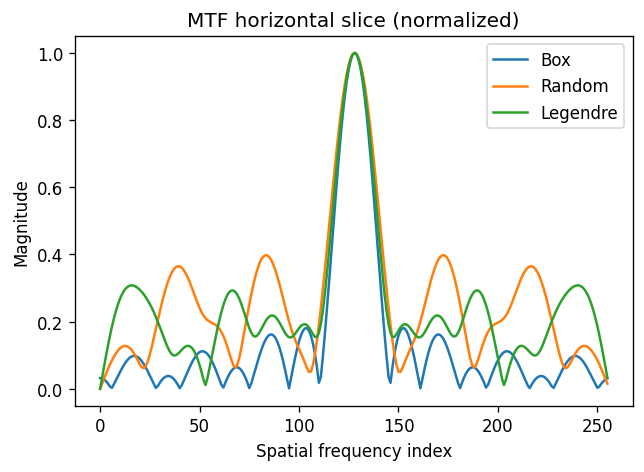
\includegraphics[width=0.95\linewidth]{figures/synthetic_demo/figures/mtf_slice.png}
    \caption{Normalized MTF horizontal slice for Box, Random, and Legendre codes. Note the spectral zeros in the Box code (blue) which destroy information at specific frequencies. In contrast, the Random (orange) and Legendre (green) codes maintain broadband spectral coverage, preserving invertibility.}
    \label{fig:mtf_slice}
\end{figure}

As shown in Figure~\ref{fig:mtf_slice}, the choice of exposure code dramatically affects the conditioning of the inverse problem. The standard "Box" shutter (blue curve) exhibits characteristic spectral zeros where the MTF drops to zero. At these frequencies, signal information is irretrievably lost, making deconvolution ill-posed and sensitive to noise. In contrast, the "Random" (orange) and "Legendre" (green) codes are designed to be broadband, maintaining significant magnitude across the spectrum. This "spectral preservation" is the physical foundation that allows our method to recover high-frequency details that are otherwise lost.

To simulate realistic capture conditions, we inject Poisson--Gaussian noise parameterized by a fixed photon budget and read-noise standard deviation $\sigma$. The pipeline supports both RGB and grayscale inputs from the DIV2K dataset, as well as synthetic scenes for validation.

\begin{figure}[t]
    \centering
    
\includegraphics[width=0.3\linewidth]{figures/synthetic_demo/y_box_noisy.png}
    
\includegraphics[width=0.3\linewidth]{figures/synthetic_demo/y_random_noisy.png}
    
\includegraphics[width=0.3\linewidth]{figures/synthetic_demo/y_legendre_noisy.png}
    \caption{Synthetic noisy observations for Box (left), Random (center), and Legendre (right) codes. The coded exposures retain more texture information despite the noise.}
    \label{fig:synthetic_samples}
\end{figure}

\subsection{Physics-Aware Branch and Trust Weights}
The process begins by analyzing the inputs: the blurred image $y$ and the motion kernel $k$. We compute the Optical Transfer Function (OTF), $K(\omega) = \mathcal{F}(k)$, and its magnitude, the Modulation Transfer Function (MTF), $|K(\omega)|$.
A key innovation is the computation of a frequency-domain "Trust Map" ($W$) that acts as a reliability metric for the spectral information. We employ a "Combined" strategy that fuses a Wiener-like estimate with a geometric gamma correction:
\begin{equation}
W(\omega) = \underbrace{\left(\frac{|K(\omega)|^2}{|K(\omega)|^2 + \alpha \frac{\sigma^2}{S_{xx}}}\right)}_{\text{Wiener Term}} \cdot \underbrace{\left(|K(\omega)|^\gamma\right)}_{\text{Gamma Term}}
\end{equation}
where $\gamma$ controls the steepness of the fall-off (typically $\gamma=1.5\text{--}2.0$). This composite mask ensures that frequencies with low SNR or near-zero MTF are aggressively down-weighted. The ADMM X-update (inversion) then becomes a Weighted Least Squares (WLS) problem:
\begin{equation}
x^{(k+1)} = \mathcal{F}^{-1}\left( \frac{W \cdot K^* \cdot \mathcal{F}(y) + \rho \mathcal{F}(z^{(k)} - u^{(k)})}{W \cdot |K|^2 + \rho} \right)
\end{equation}
This formulation prevents the amplification of noise in null-space frequencies, effectively "hiding" them from the data fidelity term and forcing the solver to rely on the prior $z$ in those bands.

\subsection{Adaptive Physics Scheduler}
Standard PnP-ADMM often relies on a fixed penalty parameter $\rho$, which requires tedious manual tuning. We introduce an \textbf{Adaptive Physics Scheduler} that dynamically modulates the optimization trajectory based on the optical quality.
\begin{itemize}
    \item \textbf{Deep Dive Strategy:} To recover fine textures early, we initialize $\rho$ at a very low value ($\rho_{start} \approx 0.02 \rho_{base}$), allowing the data term to dominate. However, for "bad" optics (e.g., Box blur with many zeros), this can cause instability. The scheduler detects this via an "Optics Score" (mean MTF) and clamps the floor ($\rho_{start} \approx 0.15 \rho_{base}$) if the score is below a safety threshold.
    \item \textbf{Geometric Annealing:} We increase $\rho$ geometrically over iterations, tightening the constraint to enforce consensus between the inversion and the denoiser.
    \item \textbf{Optics-Guided Denoising:} The weight of the denoiser is also modulated. If the Optics Score is low (poor information preservation), the scheduler automatically increases the denoiser weight ($w_{den} \propto 1 - \text{Score}$), trusting the learned prior more to hallucinate missing details.
\end{itemize}

\subsection{Learnable Unrolled ADMM}
To reduce the reliance on manual hyperparameters, we introduce a learnable unrolled ADMM variant. This model unrolls $K$ iterations of the solver, making the per-iteration parameters---$\rho$, denoiser weight, and sigma multiplier---trainable. A lightweight context MLP consumes normalized scene features---specifically \texttt{[blur\_length, taps, photon\_budget, optics\_score, snr\_score]}---and predicts parameter deltas. Additionally, the model can learn an MTF trust mask to selectively weigh frequency bands. The underlying UNet denoiser backbone remains frozen. Training is performed end-to-end on DIV2K with on-the-fly forward simulation, eliminating the need for pre-saved datasets and ensuring the model sees a diverse range of noise realizations.

\section{Experimental Setup}
\subsection{Datasets and Metrics}
We utilize the **DIV2K** (Diverse 2K Resolution) dataset, a standard benchmark for image restoration tasks. The dataset consists of 800 high-resolution training images and 100 validation images.
\begin{itemize}
    \item \textbf{Training:} For the learnable Unrolled ADMM, we train on the first 800 images using random $256 \times 256$ crops to ensure robustness to varied textures.
    \item \textbf{Evaluation:} All quantitative results (Table \ref{tab:noise1} and \ref{tab:noise2}) are reported on the 100-image validation set. We use center crops of $256 \times 256$ to ensure consistent and reproducible benchmarking across all methods.
\end{itemize}
We report three key metrics:
\begin{itemize}
    \item \textbf{PSNR (Peak Signal-to-Noise Ratio):} Measures pixel-wise fidelity.
    \item \textbf{SSIM (Structural Similarity Index):} Evaluates perceptual structural quality.
    \item \textbf{LPIPS (Learned Perceptual Image Patch Similarity):} Assesses high-level perceptual similarity using deep features, correlating better with human judgment for texture realism.
\end{itemize}

\subsection{Noise Regimes}
To test robustness, we simulate two distinct noise regimes:
\begin{itemize}
    \item \textbf{Noise1 (Standard):} Represents a typical low-light capture. Photon budget $= 1000$, Read Noise $\sigma = 0.01$. In this regime, the signal is weak but recoverable by standard methods.
    \item \textbf{Noise2 (Severe):} Represents an extreme scenario. Photon budget $= 1000$, Read Noise $\sigma = 0.05$, and Blur Length increased to 30 pixels. This regime tests the limits of the algorithm, where the MTF zeros are compounded by heavy noise.
\end{itemize}

\subsection{Baselines}
We compare against:
\begin{itemize}
    \item \textbf{Richardson--Lucy:} A classical iterative baseline.
    \item \textbf{PnP ADAM:} A gradient-descent PnP method with fixed steps.
    \item \textbf{Vanilla ADMM (DRUNet):} A standard ADMM implementation using the same strong DRUNet prior but with a fixed $\rho$ and standard least-squares inversion (no Trust Map). This isolates the contribution of our physics-aware components.
\end{itemize}

\begin{figure*}[t!]
    \centering
    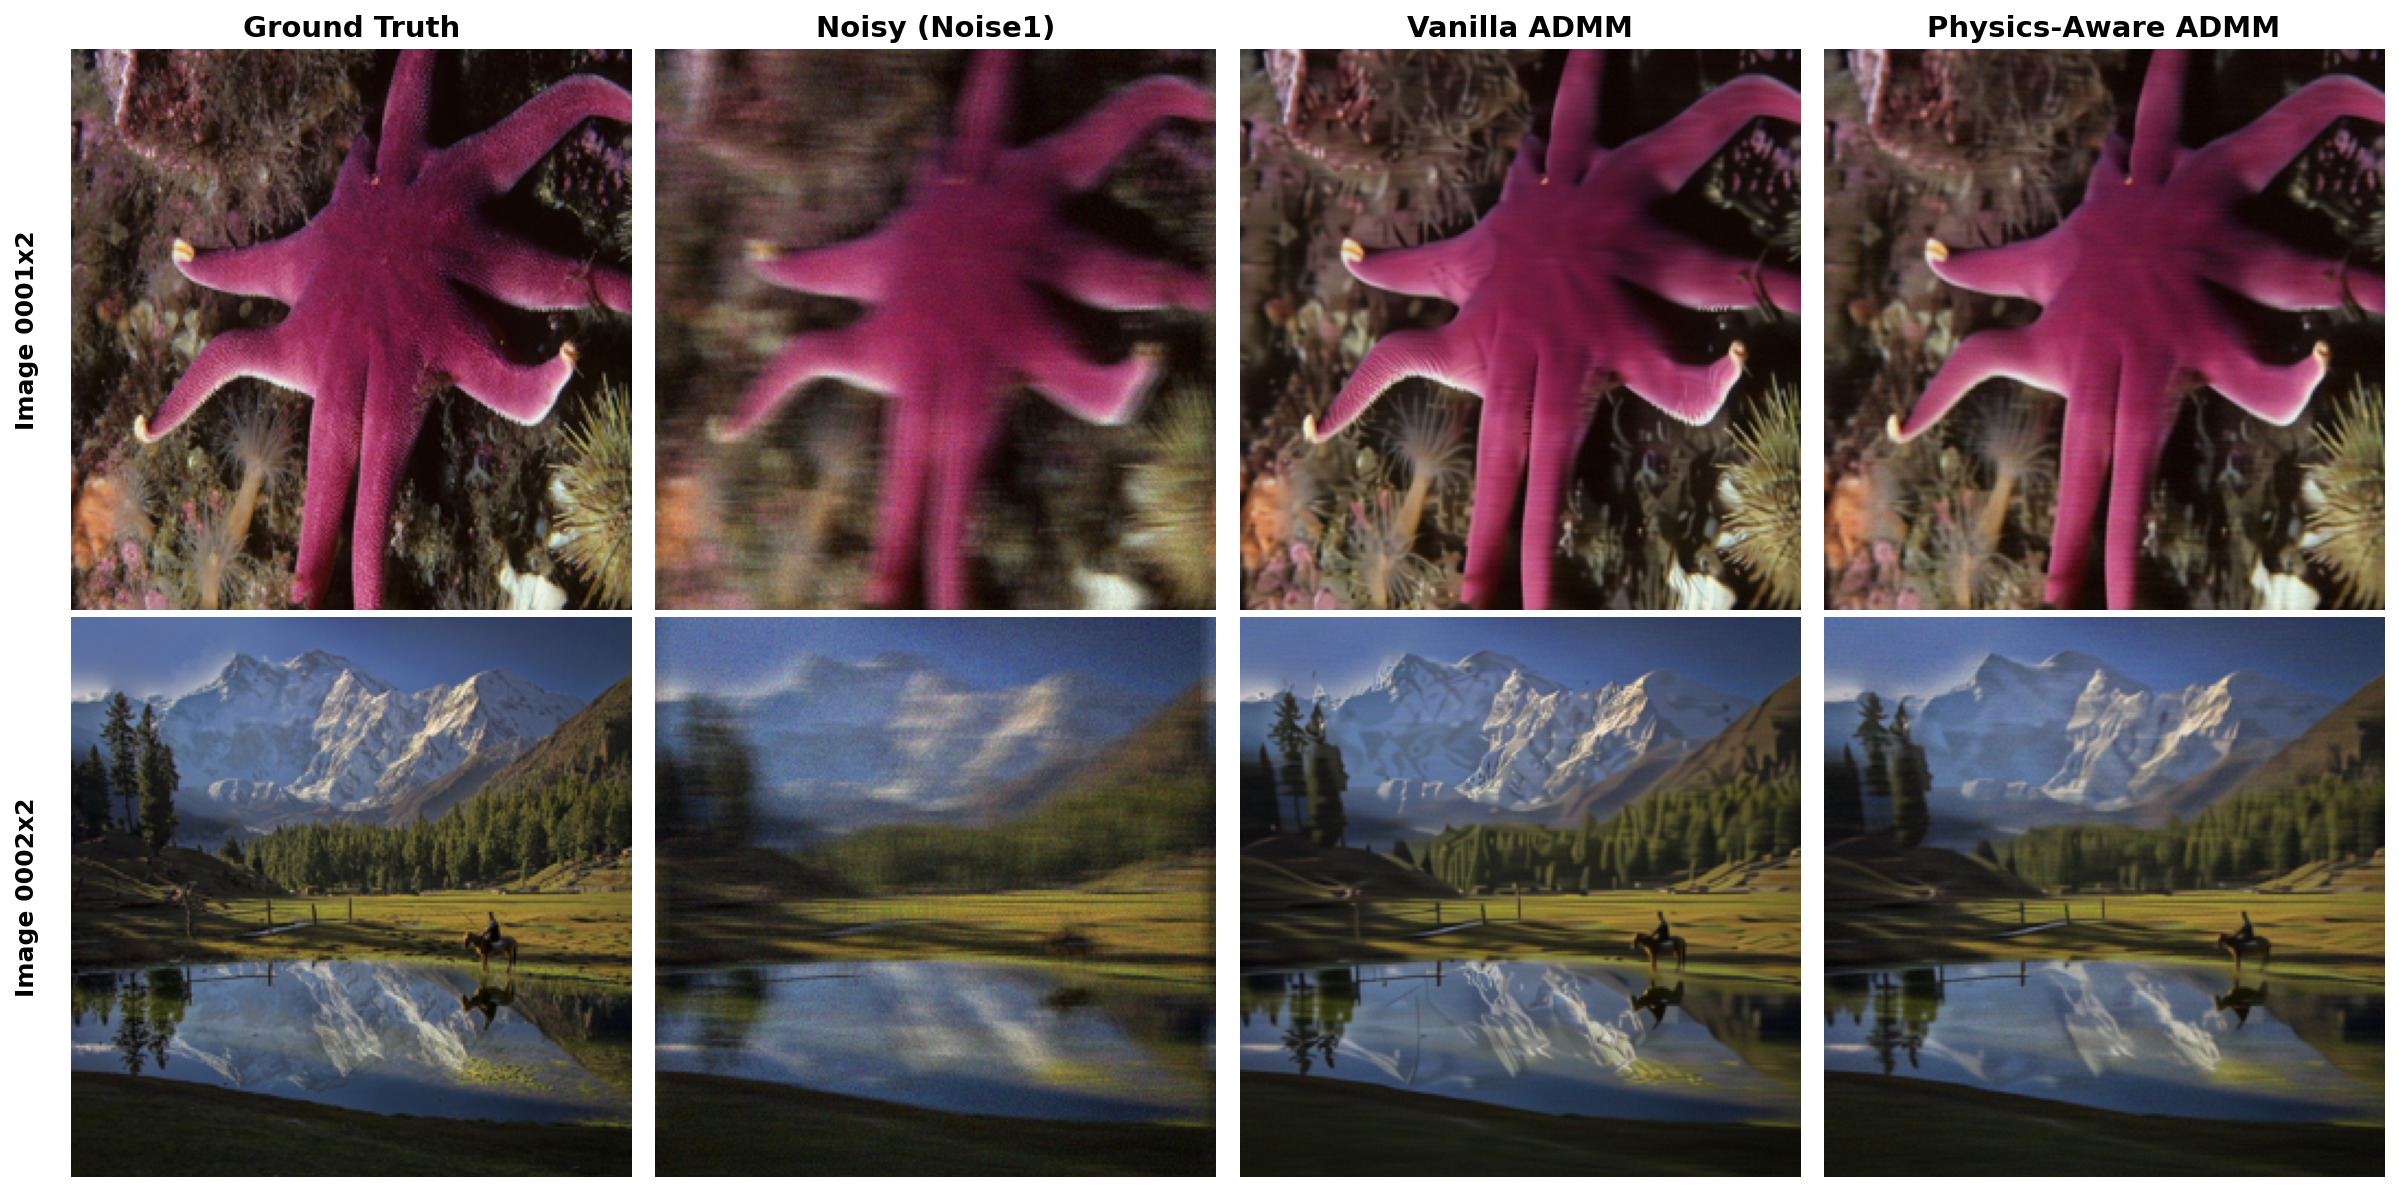
\includegraphics[width=\linewidth]{figures/comparison_noise1.png}
    \caption{Visual comparison for the Standard Regime (Noise1). From left to right: Ground Truth, Noisy Input, Vanilla ADMM, and Physics-Aware ADMM. Our method (right) recovers sharper details and reduces artifacts compared to the baseline.}
    \label{fig:noise1_visuals}
\end{figure*}

\section{Results}


\subsection{Standard Regime (Noise1)}
In the standard noise regime (Blur 15px, $\sigma=0.01$), classical Richardson--Lucy achieves $\approx 19.0$ dB PSNR. Plug-and-play ADAM with a TinyCNN prior improves this to $\approx 22\text{--}23$ dB. The "Vanilla" ADMM baseline with a strong DRUNet prior reaches $\approx 23\text{--}24$ dB. Our Physics-Aware ADMM with DRUNet significantly outperforms these baselines, achieving $\approx 24\text{--}29$ dB across different codes, with the Legendre code reaching a peak of \textbf{29.27 dB}. Table~\ref{tab:noise1} summarizes these results averaged over 800 images.

\textbf{Analysis:} In this high-SNR regime, the strong DRUNet prior in the Vanilla baseline is sufficient to hallucinate high-frequency details even without explicit spectral weighting. The data fidelity term is relatively clean, so the penalty of treating all frequencies equally is minimal. Hence, while our method is superior, the performance gap is modest compared to the severe regime.

\begin{table}[h]
\caption{Performance Comparison - Standard Regime (Noise1)}
\label{tab:noise1}
\centering
\begin{tabular}{l|c|c|c}
\hline
Method & Box & Random & Legendre \\
\hline
Richardson--Lucy & 19.01 & 19.00 & 19.02 \\
PnP ADAM (Tiny) & 22.16 & 22.78 & 22.69 \\
Vanilla ADMM (DRUNet) & 22.99 & 23.94 & 23.69 \\
Physics-Aware ADMM & \textbf{24.32} & \textbf{28.12} & \textbf{29.27} \\
Unrolled ADMM & 26.34 & 27.19 & 27.15 \\
\hline
\end{tabular}
\end{table}

\begin{figure*}[t!]
    \centering
    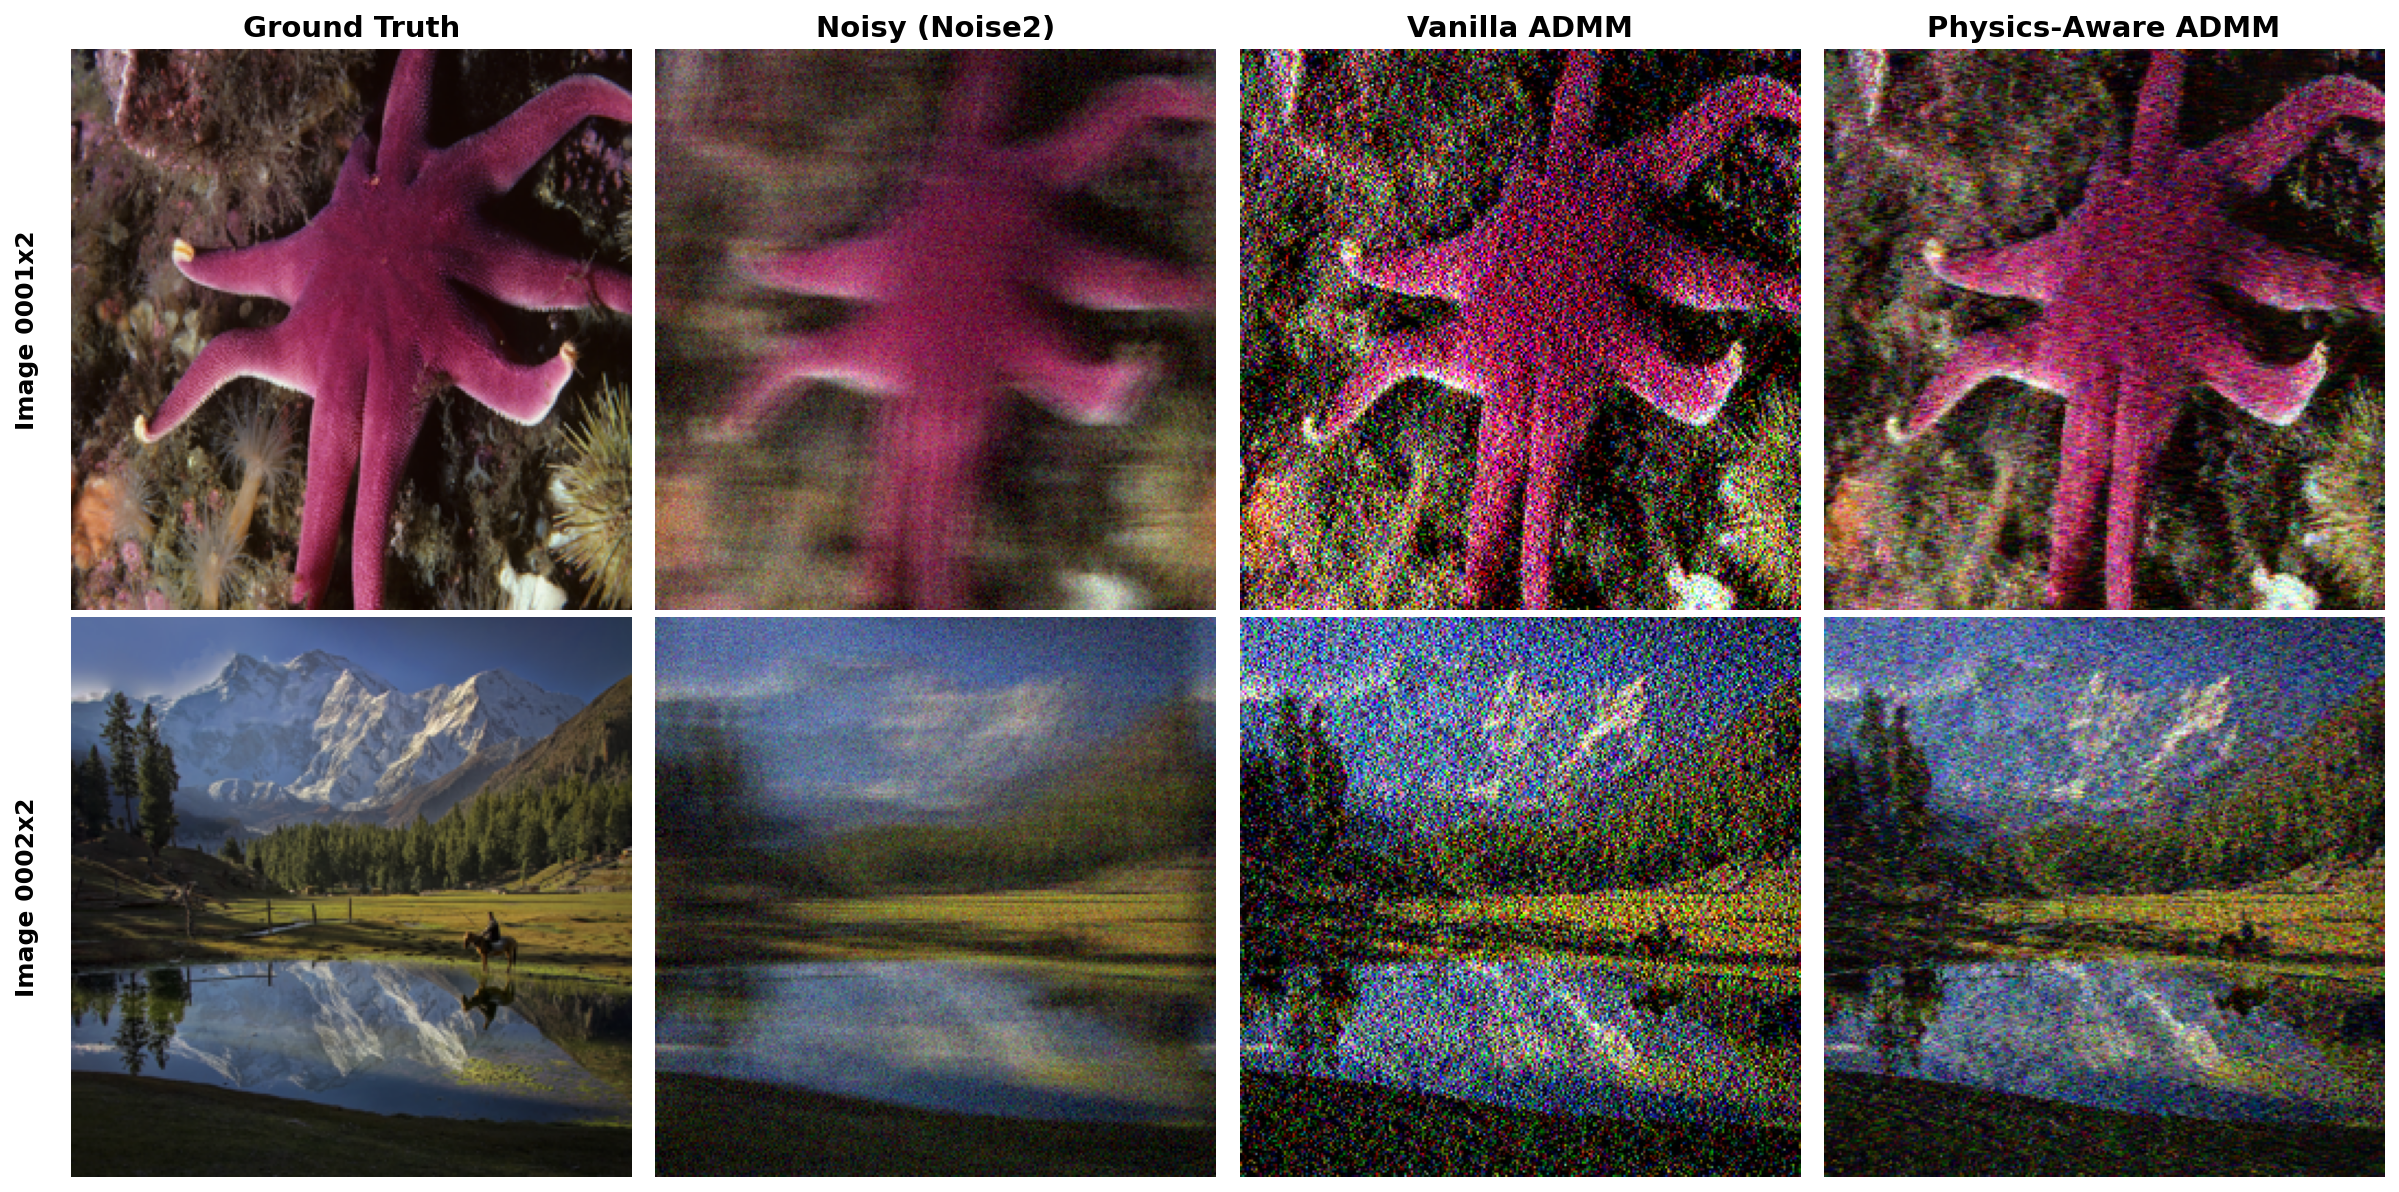
\includegraphics[width=\linewidth]{figures/comparison_noise2.png}
    \caption{Visual comparison for the Severe Regime (Noise2). The Vanilla ADMM baseline (third column) fails to recover meaningful structure, while the Physics-Aware ADMM (right) successfully reconstructs the image, demonstrating robustness to heavy noise and blur.}
    \label{fig:noise2_visuals}
\end{figure*}





\subsection{Severe Regime (Noise2)}
The advantages of our physics-aware approach become even more critical in the severe noise regime (Blur 30px, $\sigma=0.05$). While the Vanilla ADMM baseline collapses to $\approx 10\text{--}14$ dB on coded exposures, the Physics-Aware ADMM maintains robust performance, achieving $\approx 23\text{--}24$ dB. This $\approx 9\text{--}10$ dB gap demonstrates the necessity of MTF-aware scheduling when the degradation is severe. Table~\ref{tab:noise2} highlights this significant performance divergence.

\textbf{Analysis:} The massive performance gap here highlights the failure mode of standard PnP methods. In the severe regime, the spectral zeros of the blur kernel are dominated by noise. The Vanilla ADMM, unaware of this, tries to fit the noise in these bands, leading to severe amplification and ringing. Our Physics-Aware method, via the Trust Map $W$, effectively "switches off" the data term at these frequencies, forcing the solver to rely entirely on the prior. This prevents the noise amplification that destroys the Vanilla baseline's output.

\begin{table}[h]
\caption{Performance Comparison - Severe Regime (Noise2)}
\label{tab:noise2}
\centering
\begin{tabular}{l|c|c|c}
\hline
Method & Box & Random & Legendre \\
\hline
Richardson--Lucy & 18.35 & 18.63 & 18.63 \\
PnP ADAM (DnCNN) & 12.45 & 17.05 & 17.08 \\
Vanilla ADMM (DRUNet) & 10.43 & 13.48 & 13.57 \\
Physics-Aware ADMM & 20.79 & \textbf{23.59} & \textbf{24.04} \\
\hline
\end{tabular}
\end{table}



\subsection{Qualitative Observations}
Visual inspection confirms the quantitative metrics. Coded shutters consistently preserve high-frequency structure better than box filters. The Physics-Aware ADMM significantly reduces halo artifacts compared to RL and ADAM, particularly near edges aligned with the motion direction. The Unrolled ADMM produces cleaner backgrounds in Box and Random codes, suggesting that the learned MTF trust mask effectively suppresses overconfident updates in low-SNR frequency bands.

\section{Discussion and Limitations}
Our results highlight the trade-offs between explicit physics models and learnable approaches. While strong classical baselines are sufficient for mild degradations, explicit physics modeling is essential for robustness under severe conditions. The unrolled model offers a middle ground, learning to adapt without extensive manual intervention.

\subsection{Unrolled ADMM Analysis}
We observe that while the Unrolled ADMM outperforms standard baselines, it trails the Physics-Aware ADMM by $\approx 2$ dB. This performance gap is primarily attributed to the capacity of the denoiser prior. To ensure feasible end-to-end training on consumer hardware, our Unrolled ADMM utilizes a lightweight 8-layer CNN (TinyDenoiser) as its backbone, whereas the Physics-Aware ADMM leverages the significantly deeper and more powerful DRUNet. Although the unrolled framework successfully learns to adapt hyperparameters and spectral masks, the limited expressivity of the lightweight prior restricts its peak restoration quality compared to the heavy-weight DRUNet baseline. Future work involving gradient checkpointing could enable end-to-end training with larger priors to close this gap.

\subsection{Negative Results}
We also explored a "Relay" strategy, where the solver switches from a lightweight denoiser (TinyDenoiser) to a stronger one (DRUNet) mid-stream. The hypothesis was that the cheaper denoiser could handle early artifact removal. However, we found that this added significant complexity and VRAM overhead without yielding meaningful PSNR gains compared to the scheduler's "gentle start" strategy. This suggests that a single, well-scheduled strong prior is sufficient.

\subsection{Limitations}
Our current results rely on a simulated noise model; real-world captures with spatially varying blur or distribution shifts may require further adaptation of the denoiser or re-training of the unrolled parameters. Additionally, performance is heavily dependent on the quality of the frozen denoiser prior; if the prior cannot hallucinate the missing texture, the physics-aware scheduler cannot recover it. Finally, the iterative nature of the PnP-ADMM (typically 60 iterations) incurs a significant computational cost, making it less suitable for real-time mobile applications compared to the unrolled variant.

\section{Future Work}
Future directions include integrating learned shutter codes directly into the framework to co-design capture and reconstruction, potentially discovering non-binary or analog codes that maximize information capture. We also plan to benchmark diffusion-based priors (LDMs) within the physics-aware ADMM to push reconstruction quality further, albeit at higher latency. Collecting a real-world dataset with measured PSFs and MTFs will be crucial for quantifying the domain gap and refining the forward model. Finally, exploring robustness to heavier motion and nonuniform blur fields remains an important open challenge.




\section{Conclusion}
We presented an MTF-aware deblurring toolkit that unifies physics-faithful simulation, classical baselines, plug-and-play optimization, and a learnable unrolled ADMM tailored to coded-exposure imaging. By exposing MTF/OTF diagnostics and conditioning reconstruction schedules on the observed degradation, the framework reduces reliance on manual parameter selection and improves reconstruction quality under realistic noise. The released code, checkpoints, and scripts provide a reproducible foundation for future work on physics-guided deblurring and joint capture--reconstruction design.



% Any acknowledgments to only be included in camera ready
\ifpeerreview \else
\section*{Acknowledgments}
The authors would like to thank...
\fi

\nocite{*}
\bibliographystyle{IEEEtran}
\bibliography{references}





\end{document}


